\section{System Overview}
\label{sec:system}

\begin{figure}[t]
        \centering
        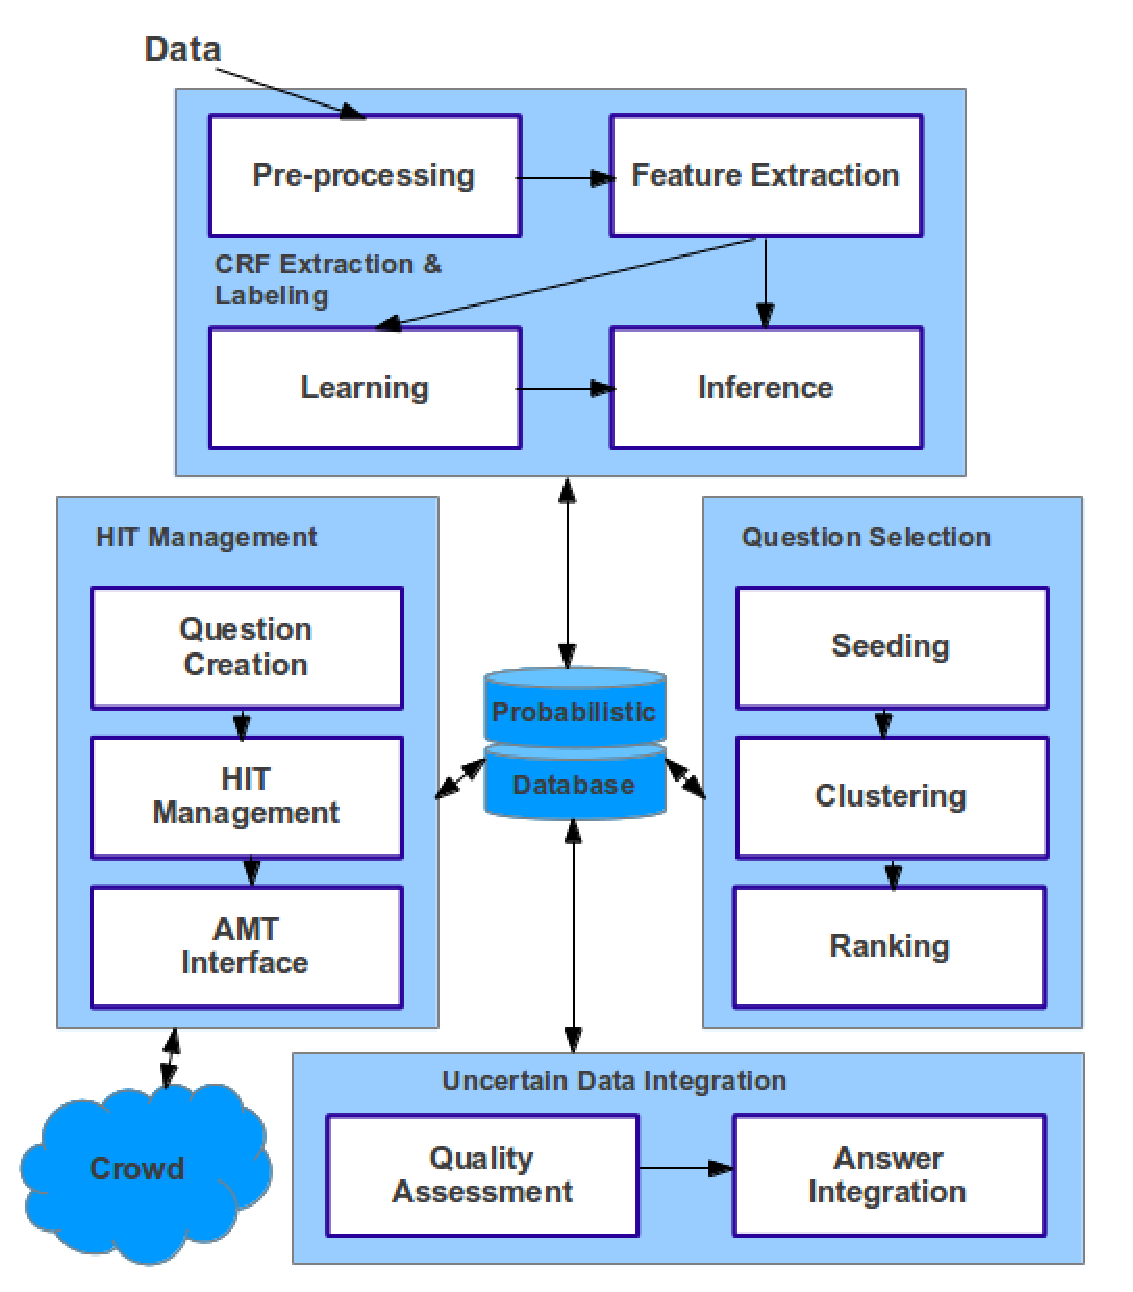
\includegraphics[width=.9\textwidth]{architecture.eps}
        \caption{Architecture of the \sysName system.}
        \label{fig:system}
\end{figure}

Figure~\ref{fig:system} outlines the basic architecture of the \sysName system, which is comprised of four main components: 1. CRF Extraction \& Inference, 2. Question Selection, 3. HIT Management, and 4. Uncertain Data Integration. The arrows chart the flow of data within and between different components. Overall, data flows through the four components in order. First, SML models are applied to perform automatic text extraction and labeling. The uncertain extractions are stored in a probabilistic database. Second, a set of ranked questions are selected from uncertain IE results. Third, the HIT manager formulates and pushes these questions to the crowd and retrieves the answers. Fourth, the Turker answers are combined probabilistically and integrated back into the database, improving the initial IE results from the CRF.

In this section we briefly outline each of the system's components and how they are related, as well as how data is specifically stored in the data model.
While we use existing techniques for 1. CRF Extraction and 3. HIT Management, we develop novel techniques for 2. Question Selection and 4. Uncertain Data Integration in Section~\ref{sec:selection} and Section~\ref{sec:integration}.

\subsection{Feature Extraction \& Inference}

The initial extraction and labeling of unstructured text is handled by the Extractor \& Inference module.  Parameter estimation
(learning) of the model is done in advance using a labeled data set. Maximum likelihood labels and marginal probabilities can be inferred from the CRF model and the uncertain label or extraction tables in a probabilistic database. We adopt the probabilistic data model outlined in~\cite{DBLP:journals/pvldb/WangFGH10}.

Unstructured text is treated as a set of documents or text-strings $\mathcal{D}$.  Each document $d \in \mathcal{D}$ has a substructure comprising a set of tokens $t^{d}_{i}$, where $i \in \{1, \dots, N\}$ and $N$ is the length of the string (document). These tokens are stored in the relational format with attributes (\emph{docID, pos, token}). In addition, a probabilistic attribute label$^{p}$ is also included, whose value can be inferred by the model. The schema of the uncertain IE results generated from the CRF is: \

\begin{figure*}[t]
        \centering
	\setlength\fboxsep{0pt}
	\setlength\fboxrule{0.5pt}
        \fbox{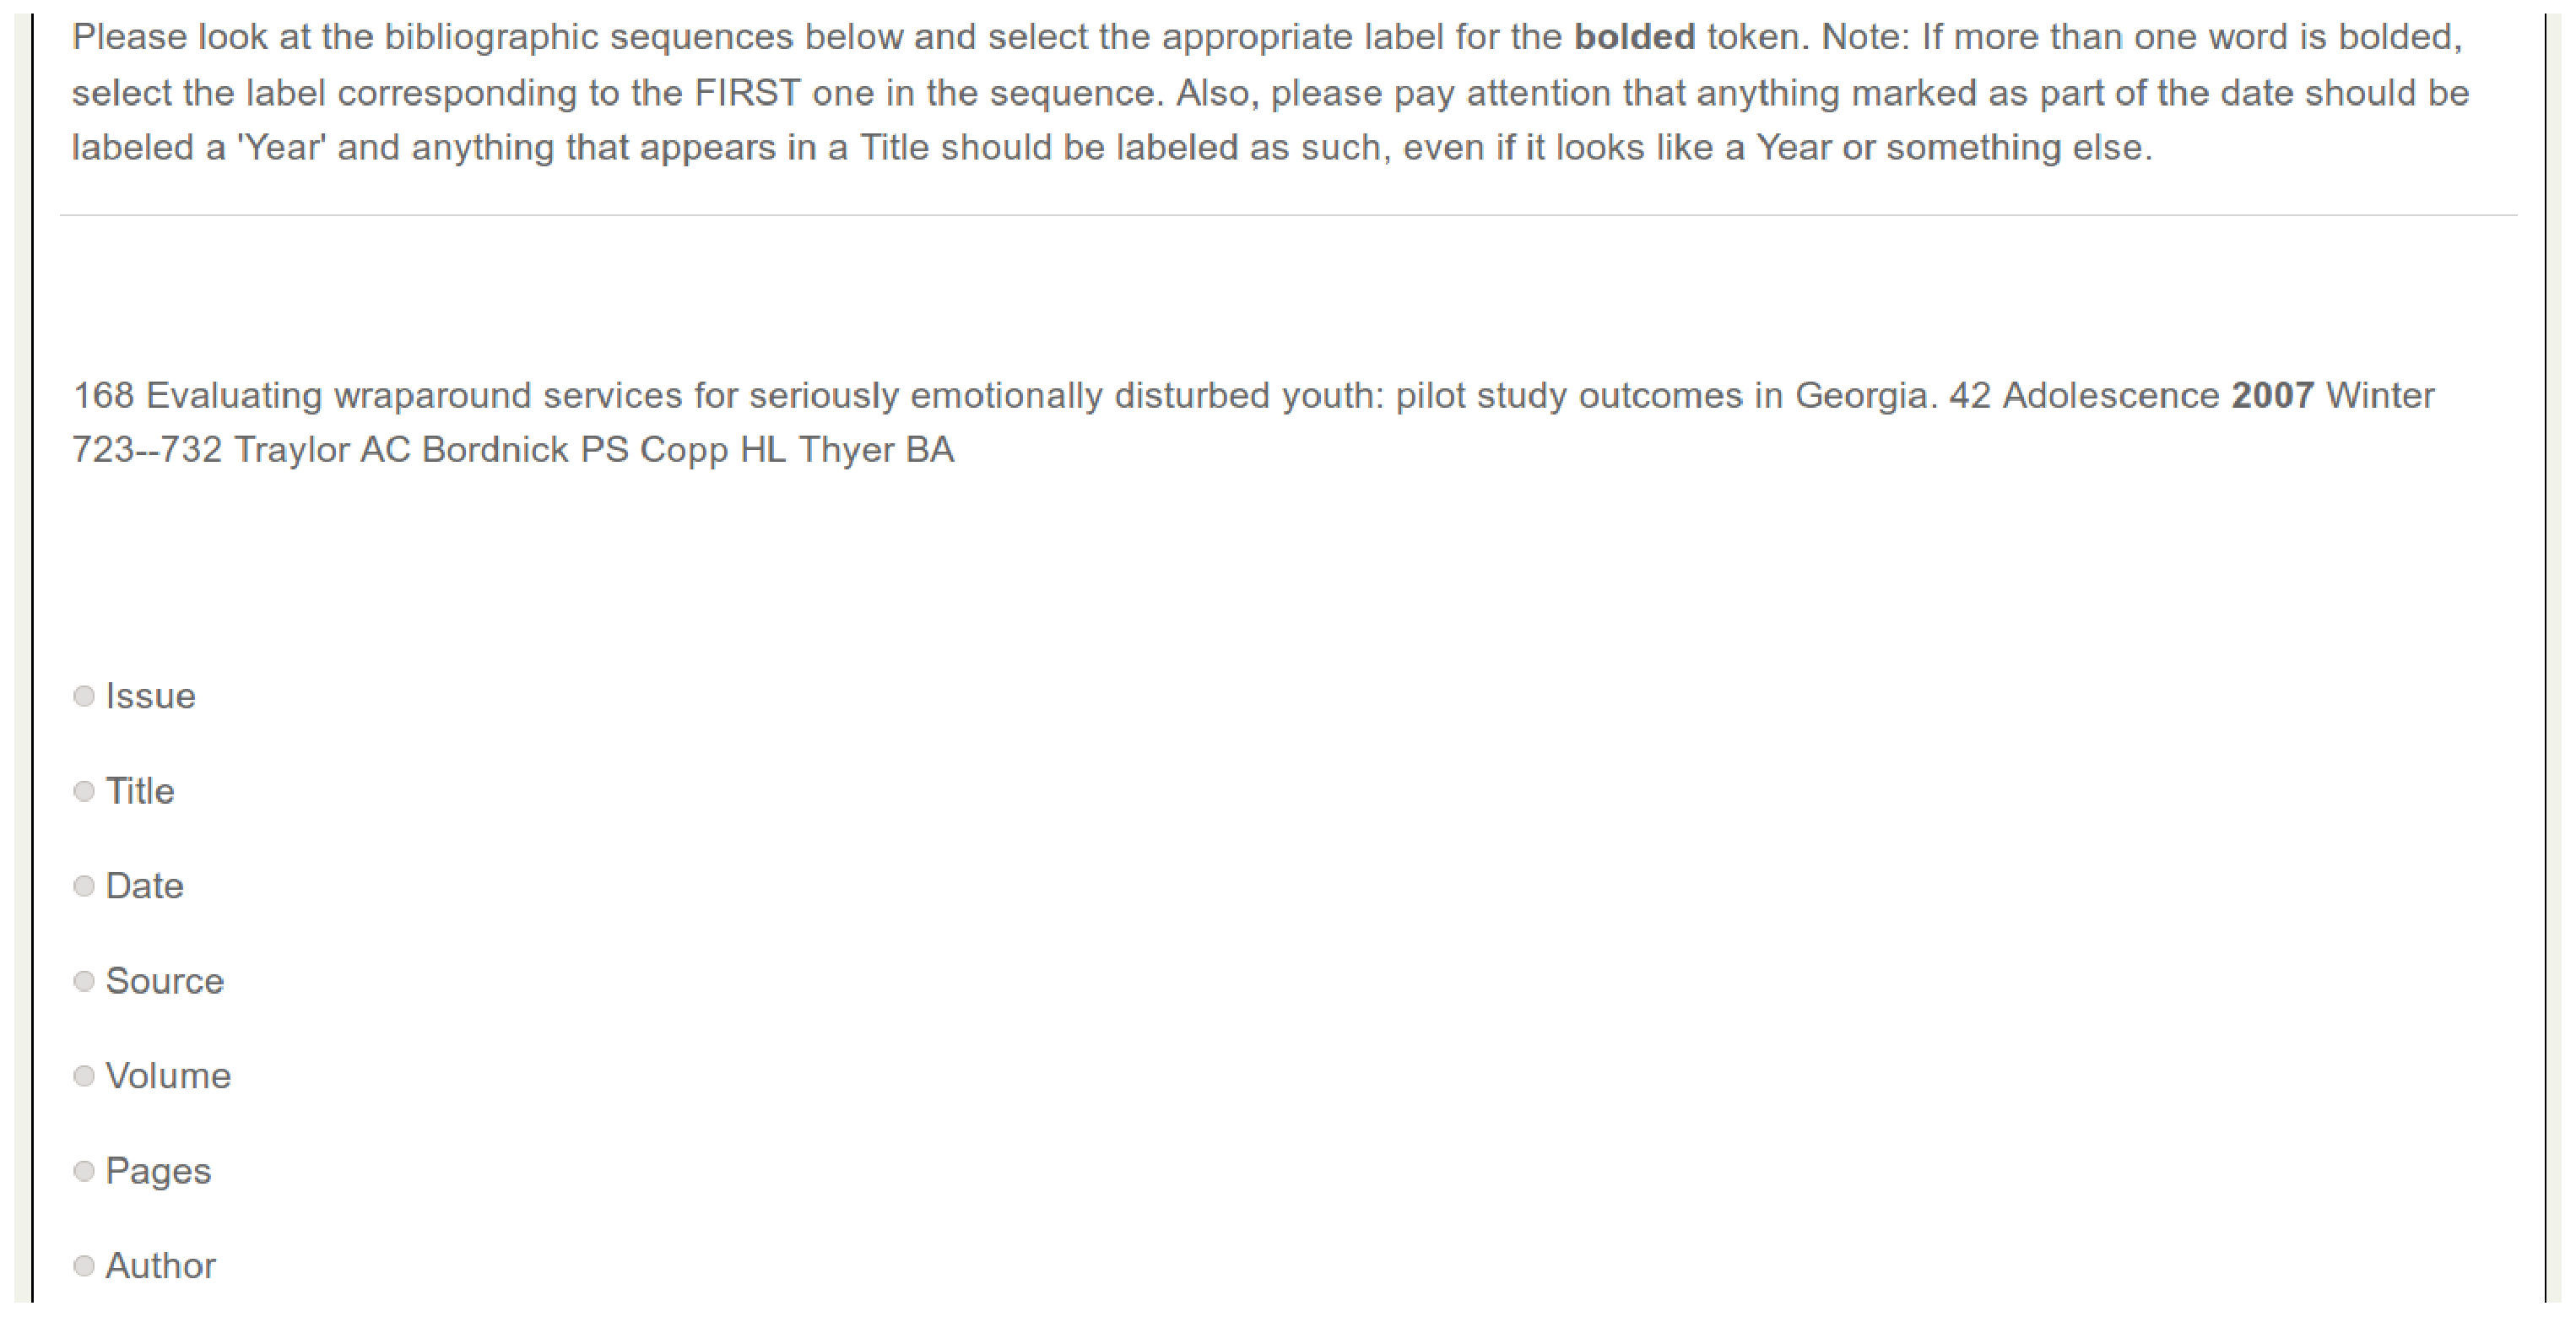
\includegraphics[width=.95\textwidth]{interface.eps}}
        \caption{Sample Mechanical Turk HIT Interface}
        \label{fig:HIT_int}
\end{figure*}

\vspace{.1in} \centerline{C{\small RF}L{\small BL}T{\small BL}(docID, pos, token, label$^{p}$)} \vspace{.1in}

The probabilistic label attribute label$^{p}$ maps to a random variable within a grounded CRF model.  Queries such as MARGINAL and TOP-K extraction can be run over the collection of probabilistic labels.

\subsection{Question Selection}

The novelty of \sysName is that it improves the results of automatic text labeling and extraction with additional evidence collected from the crowd.  Utilizing data uncertainty information, it automatically selects questions over tokens that are more uncertain and likely to contain errors. This process of \textit{Question Selection} is illustrated by the right-hand module in Figure~\ref{fig:system}, which applies three consecutive techniques over the uncertain C{\small RF}L{\small BL}T{\small BL} table: Filtering, Clustering, and Ranking. Filtering selects an initial set of tokens to be corrected based on mutual information; Clustering, groups those filtered tokens with similar attributes together using a trigram contextual model to reduce redundancy; Ranking, performs a total ordering over token clusters.  Cluster assignments and rankings for all tokens passing the initial Filtering operation are stored in a selection table.

\vspace{.1in} \centerline{S{\small ELECTION}T{\small BL} (docID, pos, clusterID, ranking)} \vspace{.1in}

The selection of questions is performed with a fixed budget and optimized for the cost of each question.
We focus on uniform, fixed-cost questions, though our methods may be easily extended to multiple question types incurring different costs.

%Assuming the labeling of a single token can be mapped to a single AMT question, \textit{seeding} generates the initial set of candidate tokens. These seeded tokens, if translated into questions and labeled by humans, would be more informative than the rest of the tokens. We use information theory and entropy to select this first batch of candidates. The selected tokens are then \textit{clustered} by similarity to find cases where a single question can resolve multiple errors or uncertainty. The intuition is that we should ask different enough questions to reduce the information overlap between questions. Finally, candidate tokens are ranked by the information gain, which is estimated by the token entropy and the token cluster. The \topk tokens selected are stored into a selection table.



\subsection{HIT Management}

The HIT manager has the responsibility of taking the rows of S{\small ELECTION}T{\small BL}, converting them into AMT questions (i.e., HITs), and posting those questions onto Amazon Mechanical Turk. The Question Creation subcomponent generates an XML template for a multiple choice question for each selected token. An example interface is shown in Figure~\ref{fig:HIT_int}. The entire text document (in this case a citation) is shown and the queried token is bolded.  Users select from the set of all labels the one they believe belongs to the bolded token. The Question Creator has the ability to assign multiple questions to a single HIT, this ensures Turkers answer the same subsets of questions.

The HIT manager also allows an administrator to set specifics such as the price of each HIT, length of posting, and the number of Turkers assigned to each HIT.  There is an AMT interface that uses an API to handle both the posting of questions and retrieval of answers. Both questions and answers are recorded and stored in their corresponding base tables, the primary key being a HITID supplied by Amazon when posting.

\vspace{.1in}
\centerline{P{\small OST}T{\small BL}(docID, pos, HITID)}
\vspace{.1in}

\centerline{T{\small URKER}L{\small BL}T{\small BL}(HITID, workerID, label)}
\vspace{.1in}

\subsection{Uncertain Data Integration}

The goal of integration in \sysName is to use both the crowd supplied labels and the machine generated labels to infer the annotation distribution. The first step is to assess the quality of each Turker using the well-documented method introduced by Dawid \& Skene~\cite{1979}.  This tells us how to appropriately weight Turkers of various quality in the integration process.

\vspace{.1in}
\centerline{T{\small URKER}C{\small ONF}T{\small BL}(workerID, quality)}
\vspace{.1in}

\sysName employs a novel probabilistic model for uncertain data integration over crowdsourced answers using the machinery of Bayesian conditional probability.  The CRF annotation (Section~\ref{sec:pi-crf}) is a prior and human edits from T{\small URKER}L{\small BL}T{\small BL} weighted by values in T{\small URKER}C{\small ONF}T{\small BL} are treated as additional evidence to yield a posterior annotation distribution.

\vspace{.1in}
\centerline{C{\small RWD}L{\small BL}T{\small BL}(docID, pos, label$^{p}$)}
\vspace{.1in}

As a last step, the responses in C{\small RWD}L{\small BL}T{\small BL} are integrated into the probabilistic database by constraining the node's marginal probability to the combined posterior.  Performing constrained inference has the ability to correct additional token labels based on correlations in the CRF model, further improving overall accuracy.  In the next two sections, we go into details of the new techniques developed for question selection and uncertain data integration.

\eat{The final text label table contains evidence both from CRF and the crowd.

\vspace{.1in} \centerline{C{\small ASTLE}T{\small BL}(docID, pos, token, label$^{p}$)} \vspace{.1in}
}
